\documentclass[a4paper,14pt]{extarticle}
\usepackage{color}
\usepackage{amsmath}
\usepackage{amsthm}
\usepackage{amssymb}
\usepackage{bbold}
\usepackage{mathtools}
\usepackage{centernot}
\usepackage{tikz}
\usepackage{tikz-cd}
\usepackage{caption}

\theoremstyle{definition}
\newtheorem*{theorem}{Theorem}
\newtheorem*{definition}{Definition}
\newtheorem*{lemma}{Lemma}
\newtheorem*{corollary}{Corollary}
\newtheorem*{proposition}{Proposition}
\newtheorem*{eg}{Example}

\begin{document}


\title{\textbf{Algebraic Topology - MATH0023}}
\author{\textbf{Based on lectures by Prof FEA Johnson}\\ Notes taken by Imran Radzi}
\date{}
\maketitle

\pagenumbering{roman}
Notes based on the Autumn 2021 Algebraic Topology lectures by Prof FEA Johnson.
\begingroup
\let\cleardoublepage\clearpage
\tableofcontents
\endgroup
\newpage
\pagenumbering{arabic}

\vspace{12pt}

\section{Simplicial complexes}

\begin{definition}[Simplicial complex]
	A \emph{simplicial complex} $X$ is a pair $(V_X,\mathcal{S}_X)$ where $V_X$ denotes the vertex set of $X$ and $\mathcal{S}_X$ is the set of
	\textit{finite, non-empty} subsets of $V_X$ satisfying
	\begin{enumerate}
		\item $\forall v\in V_X$, then $\{v\}\in\mathcal{S}_X$
		\item If $\sigma\in\mathcal{S}_X, \,\tau\subset\sigma, \,\tau\neq\emptyset$, then $\tau\in\mathcal{S}_X$. 
	\end{enumerate}
	$\mathcal{S}_X$ is called the set of \textit{simplices} of $X$.
\end{definition}

\begin{eg}
	A \emph{standard 1-simplex}, denoted by $\Delta^1$ is simply the line segment (or usually denoted by $I$). 
	\[V_{\Delta^1}=\{0,1\}\] \[\mathcal{S}_{\Delta^1}=\{\{0\},\{1\},\{0,1\}\}\]
	\begin{center}
	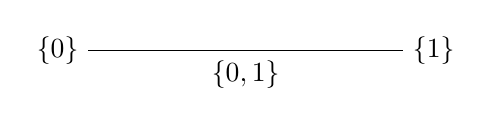
\begin{tikzpicture}
		\draw (-2,0) node[left] {$\{0\}$} node[midway,below] {$\{0,1\}$} -- (2,0) node[right] {$\{1\}$} ;
	\end{tikzpicture}
	\end{center}

\vspace{12pt}

	A \emph{standard 2-simplex}, denoted by $\Delta^2$ is the equilateral triangle.
	\[V_{\Delta^2}=\{0,1,2\}\] \[\mathcal{S}_{\Delta^2}=\{\{0\},\{1\},\{2\},\{0,1\},\{0,2\},\{1,2\},\{0,1,2\}\}\]
	\begin{center}
	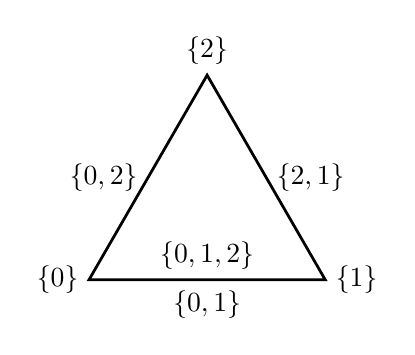
\begin{tikzpicture}
		 \draw [line width=1pt] (0,0) node[left] {$\{0\}$} -- (60:3) node[above] {$\{2\}$}  node[midway,left] {$\{0,2\}$}
		-- (3,0) node[right] {$\{1\}$} node[midway,right] {$\{2,1\}$} -- cycle node[midway,below] {$\{0,1\}$} node[midway, above]{$\{0,1,2\}$};
	\end{tikzpicture}
	\end{center}

	In general, the \emph{standard $n$-simplex} $\Delta^n$, is $\Delta^n=(V_{\Delta^n},\mathcal{S}_{\Delta^n})$ where
	\[V_{\Delta^n}=\{0,1,\ldots,n\}\] \[\mathcal{S}_{\Delta^n}=\{\alpha:\alpha\subset\{0,\ldots,n\}, \,\alpha\neq\emptyset\}\]
\end{eg}

\vspace{12pt}

\noindent If $X=(V_x,\mathcal{S}_X)$ is a simplicial complex, we now want to pick a field $\mathbb{F}$, usually $\mathbb{Q}$ or $\mathbb{F}_2$ (in this course) and want to produce a sequence of vector 
spaces (over $\mathbb{F}$)

\[C_n(X)_{0\leq n}\]

$C_0(X)$ is the vector space whose basis elements are simply the vertices of the simplicial complex, and this has dimension 0.

\begin{definition}[$k$-simplex of a simplicial complex]
	If $X$ is a simplicial complex then a \emph{$k$-simplex of $X$} is a simplex $\sigma\in\mathcal{S}_X$ such that $|\sigma|=k+1$.
\end{definition}

\noindent $C_k(X)$ is the vector space whose basis elements are the \emph{oriented} $k$-simplices of $X$ which are the following symbols,
\[[v_0,v_1,\ldots,v_n]\] (where  $\{v_0,\ldots,v_n\}$ is an $n$-simplex of $X$) subject to the rules \[[v_{\rho(0)},v_{\rho(1)},\ldots,v_{\rho(n)}]=\text{sign}(\rho)[v_0,\ldots,v_n]\]

\begin{definition}
	\[\partial_n:C_n(X)\rightarrow C_{n-1}(X)\] is a linear map defined on basis elements as follows;
	\[\partial_n[v_0,\ldots,v_n]=\sum_{r=0}^n(-1)^r[v_o,\ldots,\hat{v_r},\ldots,v_n]\] where $\hat{v_r}$ indincates omission of $v_r$.
\end{definition}

\begin{eg}
	\[\partial_2[0,1,2]=[1,2]-[0,2]+[0,1]\]
	\[\partial_1[v_0,v_2]=[v_1]-[v_0]\]
	\begin{eqnarray*}
		\partial_1\partial_2[0,1,2]&=&\partial_1([1,2]-[0,2]+[0,1]) \\
					&=&([2]-[1])-([2]-[0])+([1]-[0]) \\
					&=&0
	\end{eqnarray*}
\end{eg}

\begin{proposition}[Poincaré lemma]
	Let $X$ be a simplicial complex. Consider \[\partial_r:C_r(X)\rightarrow C_{r-1}(X)\] for $r\geq1$, then \[\partial_{n-1}\partial_n\equiv 0\]
\end{proposition}

\begin{proof}
	\begin{eqnarray*}
		\partial_n[v_0,\ldots,v_n]=\sum_{r=0}^n(-1)^r[v_0,\ldots,\hat{v_r},\ldots,v_n]
	\end{eqnarray*}

	\begin{eqnarray*}
		\partial_{n-1}[v_0,\ldots,\hat{v_r},\ldots,v_n]&=&\sum_{s<r}(-1)^s[v_0,\ldots,\hat{v_s},\ldots,\hat{v_r},\ldots,v_n] \\
									&&+\sum_{s>r}(-1)^{s-1}[v_0\ldots,\hat{v_r},\ldots,\hat{v_s},\ldots,v_n]
	\end{eqnarray*}

	\begin{eqnarray*}
		\partial_{n-1}\partial_n[v_0,\ldots,v_n]&=&\sum_{s<r}(-1)^{r+s}[v_0,\ldots,\hat{v_s},\ldots,\hat{v_r},\ldots,v_n] \\
								&&+\sum_{s>r}(-1)^{r+s-1}[v_0,\ldots,\hat{v_r},\ldots,\hat{v_s},\ldots,v_n] \\
								&=&0
	\end{eqnarray*}
\end{proof}

\begin{proposition}
	If \[C_{n+1}\xrightarrow{\partial_{n+1}}C_n\xrightarrow{\partial_n}C_{n-1}\] then \[\text{im}(\partial_{n+1})\subset\ker(\partial_n)\]
\end{proposition}

\begin{proof} By previous lemma.
\end{proof}

\section{Homology}
\subsection{Quotient spaces}
Let $V$ be a vector space over a field $\mathbb{F}$, and $U\subset V$ a vector subspace.

\begin{definition}
The following set \[x+U=\{x+u:u\in U\}\] is called the (left) coset of $U$ in $V$. Note that \[x+U=x'+U\iff x-x'\in U\]	
\end{definition}

\begin{definition}[Quotient space]
	The quotient space $V/U$ is the set \[V/U=\{x+U:x\in V\}\] where addition and scalar multiplication is defined by \[(x+U)+(y+U)=x+y+U\]\[\lambda\cdot(x+U)=\lambda x+U\] and 0 is
	represented by \[0+U\] Note that $V/U$ is a vector space.
\end{definition}

\begin{proposition}
	\[\dim(V/U)=\dim(V)-\dim(U)\]
\end{proposition}

\begin{proof}
	There exists a natural linear map \[\eta:V\rightarrow V/U\] given by \[\eta(x)=x+U\] Clearly this map is surjective so \[\dim(V/U)=\dim(\text{im}(\eta))\] Now,
	\begin{eqnarray*}
		\ker(\eta)&=&\{x\in V:\eta(x)=U\}\\
			&=&\{x\in V:x+U=U\}
	\end{eqnarray*}
	and \[x+U=U\iff x-0\in U\iff x\in U\] so $\ker(\eta)=U$. Then, \[\dim(V)=\dim\ker(\eta)+\dim\text{im}(\eta)\] so \[\dim(V/U)=\dim\text{im}(\eta)=\dim(V)-\dim(U)\]
\end{proof}

\begin{definition}
	\[H_n(X;\mathbb{F})=\ker(\partial_n)/\text{im}(\partial_{n+1})\]
\end{definition}

We call $H_n(X;\mathbb{F}$) the \emph{$n^{\text{th}}$ homology group} of $X$ with coefficients in $\mathbb{F}$. If $\mathbb{F}=\mathbb{Q}$, then $\dim H_n(X;\mathbb{Q})$ is called
the $n^{\text{th}}$ \emph{Betti} number of $X$. \\

Consider $\Delta^3$. The set $\{0,1,2,3\}$ represents the 'middle' of the tetrahedron (inside, interior). If we exclude the middle and simply take its boundary, we have \[\partial\Delta^n=S^{n-1}\]
It happens that $S^2$ (middle excluded) is the simplest simplicial model of the 2-sphere.

\begin{eg}
Consider \[H_k(S^2;\mathbb{F})\] Note that \[C_n(S^2)=0\text{ for }n\geq3\] as there are no 3-simplices, so we only have to worry about
\[H_2(S^2;\mathbb{F}),H_1(S^2;\mathbb{F}),H_0(S^2;\mathbb{F})\] We proceed to calculate these from first principles. First note that $C_3(S^2)=0$. Now, (noting the order of these bases)
 $C_2(S^2)$ has basis
\[[0,1,2],[0,1,3],[0,2,3],[1,2,3]\] $C_1(S^2)$ has basis \[[0,1],[0,2],[0,3],[1,2],[1,3],[2,3]\] and lastly $C_0(S^2)$ has basis \[[0],[1],[2],[3]\]
The linear maps \[\partial_2:C_2(S^2)\rightarrow C_1(S^2)\]\[\partial_1:C_1(S^2)\rightarrow C_0(S^2)\] can both be represented by a $6\times4$ matrix and a $4\times6$ matrix respectively.

We apply $\partial_2$ and $\partial_1$ to the bases to obtain the entries to the matrices, so for example \[\partial_2([0,1,2])=[1,2]-[0,2]+[0,1]\] so the first column of the matrix representing 
$\partial_2$ is $\begin{pmatrix}1\\-1\\0\\1\\0\\0\end{pmatrix}$ Proceeding, we will obtain that
\[\partial_2=\begin{pmatrix}1&1&0&0\\-1&0&1&0\\0&-1&-1&0\\1&0&0&1\\0&1&0&-1\\0&0&1&1\end{pmatrix}\]
\[\partial_1=\begin{pmatrix}-1&-1&-1&0&0&0\\1&0&0&-1&-1&0\\0&1&0&1&0&-1\\0&0&1&0&1&1\end{pmatrix}\]
Notice that $\partial_1\partial_2=0$, which further confirms the lemma from before. Now reducing both the matrices to row reduced echelon form, we obtain
\[\begin{pmatrix}1&0&0&1\\0&1&0&-1\\0&0&1&1\\0&0&0&0\\0&0&0&0\\0&0&0&0\end{pmatrix}\] thus $\dim\ker\partial_2=1,\,\dim\text{im }\partial_2=3$
\[\begin{pmatrix}1&0&0&-1&-1&0\\0&1&0&1&0&-1\\0&0&1&0&1&1\\0&0&0&0&0&0\end{pmatrix}\] thus $\dim\ker\partial_1=3,\,\dim\text{im }\partial_1=3$
\[0\xrightarrow[\partial_3]{} C_2\xrightarrow{\partial_2}C_1\xrightarrow{\partial_1} C_0\rightarrow0\]
so now \[H_2(S^3)=\ker(\partial_2)/\text{im}(\partial_3)=\ker(\partial_2)\cong\mathbb{F}\] as $\text{im}(\partial_3)=0$, so in total, \[H_2(S^2;\mathbb{F})\cong\mathbb{F}\] Next,
\[H_1(S^2)=\ker(\partial_1)/\text{im}(\partial_2)\] Now note that \[\dim H_1(S^2)=\dim\ker(\partial_1)-\dim\text{im}(\partial_2)=3-3=0\] thus \[H_1(S^2;\mathbb{F})=0\] Next,
\[H_0(S^2)=\ker(\partial_0)/\text{im}(\partial_1)=C_0/\text{im}(\partial_1)\] and \[\dim H_0(S^2)=\dim C_0-\dim\text{im}(\partial_1)=4-3=1\] thus \[H_0(S^2;\mathbb{F})\cong\mathbb{F}\]
\end{eg}

We've shown
\[ H_k(S^2;\mathbb{F})\begin{cases} 
			      \mathbb{F} & k=0 \\
			      0 & k=1 \\
			      \mathbb{F} & k=2 \\
			      0 & k\geq3
			   \end{cases}
\]

We will soon see that this theorem generalises if \[S^n=\Delta^{n+1}\] then \[H_k(S^n)=\begin{cases}\mathbb{F}&k=0,n\\0&\text{otherwise}\end{cases}\]

\subsection{Chain complex}
\begin{definition}[Chain complex]
	Let $\mathbb{F}$ be a field. A \emph{chain complex} over $\mathbb{F}$ is \[C_*=(C_r,\partial_r)_{r\in\mathbb{N}}\] where
	\begin{enumerate}
		\item Each $C_r$ is a vector space over $\mathbb{F}$
		\item $\partial_r:C_r\rightarrow C_{r-1}$ is a linear map such that $\partial_r\partial_{r+1}=0$ for all $r$.
	\end{enumerate}
\end{definition}

If $X=(V_X,\mathcal{S}_X)$, we have defined a chain complex \[C_*(X)=(C_r(X),\partial_r)\]

Given a chain complex \[C_*(C_r,\partial_r)_{r\geq0}\] we define its \emph{homology} $H_*(C_*)$ by \[H_k(C_*)=\ker(\partial_k)/\text{im}(\partial_{k+1})\]

If $X=(V_X,\mathcal{S}_X)$ is a simplicial complex, we define \[H_k(X,\mathbb{F})=H_k(C_*(X;\mathbb{F}))\]

\subsection{Simplicial mapping}
\begin{definition}[Simplicial mapping]
	Let $X,Y$ be simplicial complexes, i.e., $X=(V_X,\mathcal{S}_X)$ and $Y=(V_Y,\mathcal{S}_Y$). A \emph{simplicial mapping} $f:X\rightarrow Y$ is a mapping of vertex sets
	$f:V_X\rightarrow V_Y$ such that \[\sigma\in\mathcal{S}_X\implies f(\sigma)\in\mathcal{S}_Y\]
\end{definition}

\begin{eg}
	Let $X=Y=\Delta^2$. Then defining $f$ by $f(0)=1,\,f(1)=2, \,f(2)=0$, it is obvious that this mapping is simplicial. \\

	Consider the following simplicial complex
	\begin{center}
	\begin{tikzpicture}
		\draw (2,0) -- (0,0) -- (0,2) -- (2,2);
		\node[below] at (0,0) {0};
		\node[above] at (0,2) {3};
		\node[above] at (2,2) {2};
		\node[below] at (2,0) {1};
	\end{tikzpicture}
	\end{center}
	and consider \[f(0)=1,\,f(1)=2,\,f(2)=3,\,f(3)=0\] This mapping is \emph{not} simplicial as $f(\{0,1\})$ is \emph{not} a simplex.
\end{eg}

Given a simplicial mapping $f:X\rightarrow Y$, we are going to produce linear maps \[H_k(f):H_k(X)\rightarrow H_k(Y)\] such that if \[g:Y\rightarrow Z\] then \[g\circ f:X\rightarrow Z\] and
\begin{enumerate}
	\item $H_k(g\circ f)=H_k(g)\circ H_k(f)$
	\item $H_k(\text{id}_X)=\text{id}_{H_k(X)}$
\end{enumerate}

\subsection{Chain mapping}
\begin{definition}
	Let \[C_*=(C_r,\partial_r^C)\]\[D_*=(D_r,\partial_r^D)\] be chain complexes. A \emph{chain mapping} $f_*:C_*\rightarrow D_*$ is a collection of linear maps \[f*=(f_r)_{r\geq0}\] where
	$f_r:C_r\rightarrow D_r$ and the following commutes
	\[
	\begin{tikzcd}
	C_r \arrow{r}{\partial_r^C} \arrow[swap]{d}{f_r} & C_{r-1} \arrow{d}{f_{r-1}} \\
	D_r\arrow[swap]{r}{\partial_r^D} & D_{r-1}
	\end{tikzcd}
	\]	
\end{definition}

Notice from the diagram that \[\partial_n^D\circ f_n=f_{n-1}\partial_n^C\]

If $g:D_*\rightarrow E_*$ is also a chain mapping, then \[(g\circ f)_n=g_n\circ f_n:C_*\rightarrow E_*\] is also a chain mapping. \[\text{id}:C_*\rightarrow C_*,
\,\,\,\text{id}_n=\text{id}_{C_n}\] is also a chain mapping. \\

\begin{proposition}
If $f:X\rightarrow Y$ is a simplicial mapping, define \[C_n(f):C_n(X)\rightarrow C_n(Y)\] by action on a basis as follows
\[C_n(f)[v_0,\ldots,v_n]=[f(v_0),\ldots,f(v_n)]\] then \[C_*(f):C_*(X)\rightarrow C_*(Y)\] is also a chain mapping.
\end{proposition}

\begin{proof}
\begin{eqnarray*}
	\partial d_n^DC_n(f)[v_0,\ldots,v_n]&=&\partial_n^D([f(v_0),\ldots,f(v_n)]) \\
		&=&\sum_{r=0}^n (-1)^r[f(v_0),\ldots,\hat{f(v_0)},\ldots,f(v_n)] \\
		&=&C_{n-1}(f)\sum_{r=0}^n (-1)^r[v_0,\ldots,\hat{v_r},\ldots,v_n] \\
		&=&C_{n-1}(f)\partial_n^C[v_0,\ldots,v_n]
\end{eqnarray*}
\end{proof}

We will often write $f_n[v_0,\ldots,v_n$ rather than $C_n(f)[v_0,\ldots,v_n]$. \\

\begin{proposition}
If $f:X\rightarrow Y,\,g:Y\rightarrow Z$ are simplicial maps, then
\[C_n(g\circ f)=C_n(g)\circ C_n(f)\]
which sometimes we will write as \[(g\circ f)_n=g_n\circ f_n\] instead.
\end{proposition}

\begin{proof}
\begin{eqnarray*}
	(g\circ f)[v_0,\ldots,v_n]&=&[(g\circ f)(v_0),\ldots,(g\circ f)(v_n)] \\
				&=&g_n[f(v_0),\ldots,f(v_n)] \\
				&=&g_n\circ f_n[v_0,\ldots,v_n]
\end{eqnarray*}
\end{proof}

\begin{proposition}
Let \[\text{id}:X\rightarrow X\] then $C_*(\text{id}):C_*(X)\rightarrow C_*(X)$ is a chain mapping.
\end{proposition}

If $C_*=(C_n,\partial_n)$ is a chain complex, define \[H_n(C_*)=\ker\partial_n/\text{im}(\partial_{n+1})\]
It is usual to write \[Z_n(C)=\ker(\partial_n)\,\,\,(\text{cycles})\] \[B_n(C)=\text{im}(\partial_{n+1})\,\,\,(\text{boundaries})\]
thus by this notation, \[H_n(C)=Z_n(C)/B_n(C)\]

If $f=(f_n),\,C_*\rightarrow D_*$ is a chain mapping, we now want to show $f$ induces a mapping
\[H_n(F):H_n(C_*)\rightarrow H_n(D_*)\]

\begin{proposition}
	If $f:C_*\rightarrow D_*$ is a chain mapping, then \[f_n(Z_n(C_*))\subset Z_n(D_*)\]
\end{proposition}

\begin{proof}
	Recall that \[f_{n-1}\partial_n^C(z)=\partial_n^D f_n(z)\] If \[z\in Z_n(C_*),\,\partial_n^C(z)=0\] then we have \[f_{n-1}\partial_n^C(z)=0\] and so
	\[\partial_n^D f_n(z)=0\] and thus \[f_n(z)\in Z_n(D_*)\]
\end{proof}

\begin{proposition}
	If $f:C_*\rightarrow D_*$ is a chain mapping, then \[f_n(B_n(C_*))\subset B_n(D_*)\]
\end{proposition}

\begin{proof}
	Note that \[f_n\partial_{n+1}^C(x)=\partial_{n+1}^D f_{n+1}(x)\] If $\beta\in B_n(C_*)$, we can write $\beta=\partial_{n+1}^C(x)$ for some $x$ and then
	\[f_n(\beta)=\partial_{n+1}^D(k)\] where $k=f_{n+1}(x)$ so \[f_n(\beta)\in B_n(D_*)\]
\end{proof}

\begin{corollary}
	If $f:C_*\rightarrow D_*$ is a chain mapping, then $f$ induces a (linear) mapping \[H_n(f):H_n(C_*)\rightarrow H_n(D_*)\]
\end{corollary}

\begin{proof}
	An element of $H_n(C_*)$ has form \[[z]=z+B_n(C_*), \,z\in Z_n(C_*)\] Now define \[H_n(f)[z]=f_n(z)+B_n(D_*)\in H_n(D_*)\] and now note that \[f_n(z)\in Z_n(D_*)\]
\end{proof}

By now it is clear if $g:D_*\rightarrow E_*, \,f:C_*\rightarrow D_*$ are chain mappings, then \[H_n(g\circ f)=H_n(g)\circ H_n(f)\] and also if $\text{id}:C_*\rightarrow C_*$ we have
\[H_n(\text{id})=\text{id}_{H_n}\]

We now formally have \[H_n(X)=H_n(C_*(X))\]

\begin{corollary}
If $X$ is a \emph{non-empty} simplicial complex, then $H_0(X;\mathbb{F})\neq0$ (for any field $\mathbb{F}$).
\end{corollary}

\begin{proof}
	As $X\neq\emptyset$, we have that $V_X\neq\emptyset$. Let $v\in V_X$ be a vertex and $*$ be the simplicial complex \[*=(\{v\},\{\{v\}\})\] so $*$ consists of one vertex
	$v$, and one $0$-simplex $\{v\}$. Now define a constant mapping \[c:X\rightarrow *, \,c(x)=v,\,\forall x\in V_X\] We also have a simplicial mapping 
	\[\iota:*\rightarrow X, \,\iota(v)=v\] so now \[c\circ\iota=\text{id}_*\] and so \[H_0(c)\circ H_0(\iota)=H_0(\text{id}_*)\] but notice that \[H_0(*)=\mathbb{F}\] since we know
	\[C_0(*)=\mathbb{F}, \,C_r(*)=0,\,r\geq1\] and thus \[H_0(c)\circ H_0(\iota)=\text{id}_\mathbb{F}\] \[c\circ\iota=\text{id}\neq0\] and now note that $c$ is surjective,
	and $\iota$ is injective. In particular \[H_0(c):H_0(X)\rightarrow\mathbb{F}=H_0(*)\] is surjective, so \[H_0(X)\neq0\]
\end{proof}























\end{document}